\begin{minipage}[t][\PosterMiddleRowHeight][t]{\PosterHalfWidth}\vspace{0pt}
  \begin{PosterPanel}{\PosterMiddleRowHeight}{5}{IN TIME: WHAT THE GRID DOES}

    \noindent\begin{minipage}[c]{252mm}\centering
      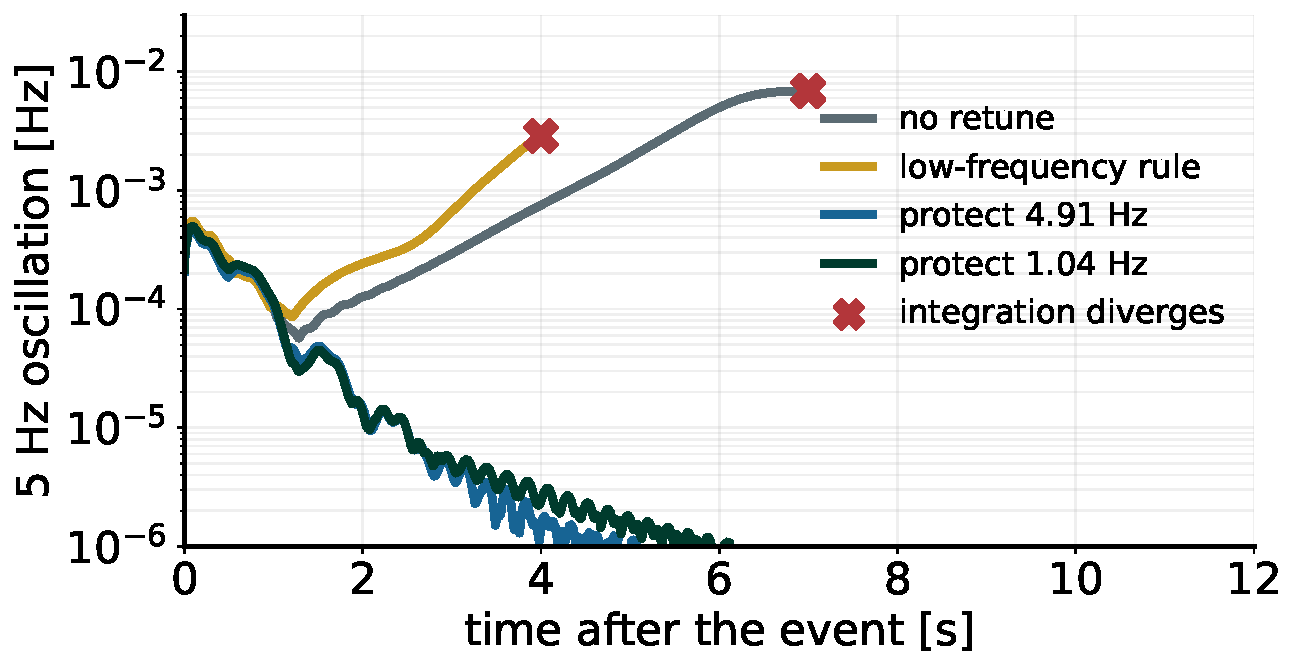
\includegraphics[width=250mm,height=112mm,keepaspectratio]{generated/figures/time_traces.pdf}
    \end{minipage}\hfill%
    \begin{minipage}[c]{166mm}\raggedright
      {\FigureSize The 5 Hz oscillation grows without a retune and with the low-frequency rule until the integration diverges. With either protected mode it dies out.\par}
    \end{minipage}\par
    \vspace{2mm}
    {\fontsize{21pt}{24pt}\selectfont Bus 16 $+100$ MW step, 44 ms at all ten PLLs. 4.2--5.6 Hz band of the bus frequencies, largest of 39 buses; below $10^{-6}$ Hz not shown. Delayed nonlinear DAE.\par}

  \end{PosterPanel}
\end{minipage}%
